\documentclass[compress]{beamer}
\usepackage[utf8]{inputenc}
\usepackage{hyperref}

\usepackage{tikz}
\usetikzlibrary{graphs, quotes, arrows.meta, matrix}

\usetheme{default}
\usecolortheme{Nord}
\setbeamertemplate{navigation symbols}{}

\title{Range query e update}
\subtitle{Segment Tree}
\author{Lorenzo Ferrari, Davide Bartoli}
\date{\today}

\begin{document}

\begin{frame}
    \maketitle
\end{frame}

\begin{frame}{Table of contents}
  \tableofcontents
\end{frame}

\section{Problema motivazionale}
\subsection{Dynamic Range Sum Queries}
\begin{frame}{Problema motivazionale}{Dynamic Range Sum Queries}
    \begin{exampleblock}{Dynamic Range Sum Queries}
        Dato un array $a$ di $n \leq 2 \cdot 10^5$ interi, processa $q \leq 2 \cdot 10^5$ delle seguenti query:
        \begin{enumerate}
            \item cambia in $u$ il valore nella posizione $k$
            \item trova la somma degli elementi nel range $[a, b]$
        \end{enumerate}
        \small{\underline{\url{https://cses.fi/problemset/task/1648}}}
    \end{exampleblock}
    \pause
    \begin{itemize}
        \item possiamo risolvere il problema in maniera naive, con update in $O(1)$ e query in $O(n)$
        \pause
        \item tenendoci l'array delle somme prefisse possiamo rispondere alle query in $O(1)$, ma ogni update costa $O(n)$
        \pause
        \item entrambe le soluzioni hanno caso pessimo $O(n q)$: al momento non sappiamo risolvere il problema efficientemente
    \end{itemize}
\end{frame}

\subsection{Sqrt Decomposition}
\begin{frame}{Problema motivazionale}{Sqrt Decomposition}
    Non possiamo ottenere complessit\`a $O(1)$ per update \textbf{e} per query. Per\`o possiamo ottenere complessit\`a minore di $O(n)$ per entrambe le operazioni.
    \pause
    \begin{block}{Sqrt Decomposition}
        \begin{itemize}
        \item dividiamo l'array in $d$ blocchi di dimensione $\frac{n}{d}$. In ogni blocco salviamo la somma dei suoi elementi
        \pause
        \item per rispondere alle query, componiamo il range $[l, r]$ come somma di blocchi e di singoli elementi. Costa in totale $O(d + \frac{n}{d})$
        \pause
        \item possiamo fare point update in $O(1)$ e range update in $O(d + \frac{n}{d})$
        \end{itemize}
    \end{block}
\end{frame}

\begin{frame}{Problema motivazionale}{Sqrt Decomposition}
    La scelta $d = \sqrt{n}$ d\`a complessit\`a $O(\sqrt{n})$/query
    \vfill
    \makebox[\textwidth]{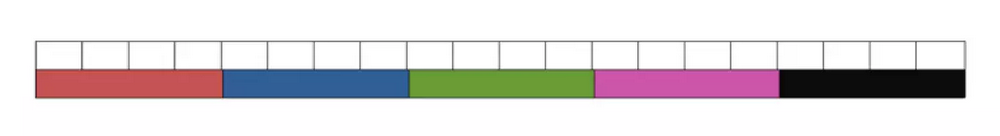
\includegraphics[scale=.3]{./img/sqrt_dec_1.png}}
    \vfill
    \begin{alertblock}{Implementazione}
        Implementando qualunque forma di Sqrt Decomposition, \textbf{non} calcolate $d = \sqrt{n}$ al momento dell'esecuzione. Dichiarare $d$ come una costante conosciuta a compile time permette al compilatore di ottimizzare molto meglio.
    \end{alertblock}
\end{frame}

\subsection{Segment Tree}
\begin{frame}{Segment Tree}{Idea}
    Ritorniamo al problema iniziale e cerchiamo di trovare un'altra soluzione.\\
    \pause
    Una possibile idea \`e quella di salvarsi la risposta per ogni possibile intervallo.\\
    \pause
    Questa soluzione per\'o non funziona perché i gli intervalli sono tanti ($O(N^2)$) e ogni update modifica la risposta di tanti intervalli.
    \pause
    Possiamo tenerci solo alcuni degli intevalli facendo in modo di riuscire a ricorstruire la soluzione per qualunque intervallo?
    \pause
    
\end{frame}

\begin{frame}{Segment Tree}{Idea}
    Proviamo a salvarci la risposta per alcuni intervalli la cui lunghezza è una potenza di $2$.    
    \vfill
    \makebox[\textwidth]{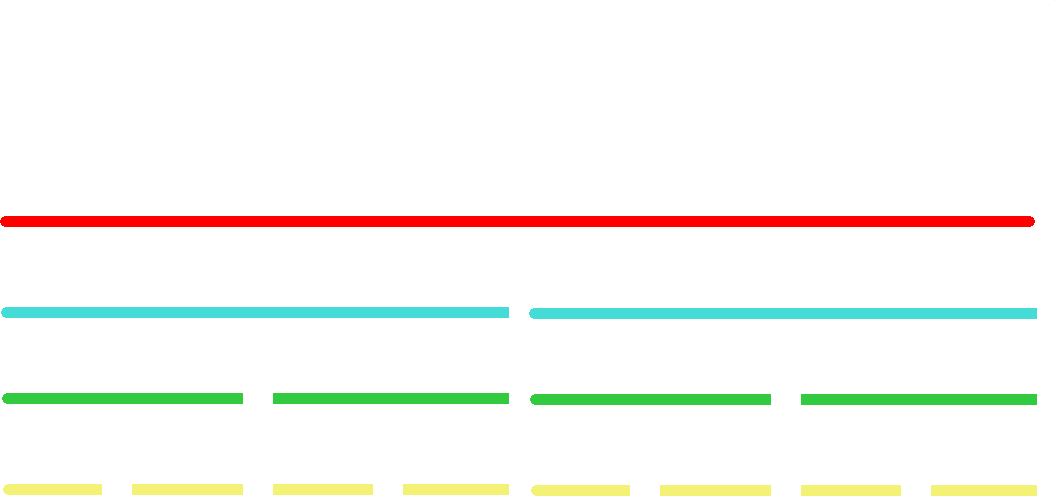
\includegraphics[scale=.70]{./img/intervalli.png}}
    \vfill
    \pause
    Quanti sono gli intervalli? \\
    $N + N/2 +N/4 ... = 2N$ \\
\end{frame}


\begin{frame}{Segment Tree}{Idea}
    Questo insieme di intervalli possiamo vederlo come un albero binario, questo ci semplificherà le cose durante l'implementazione.\\ 
    \vfill
    \makebox[\textwidth]{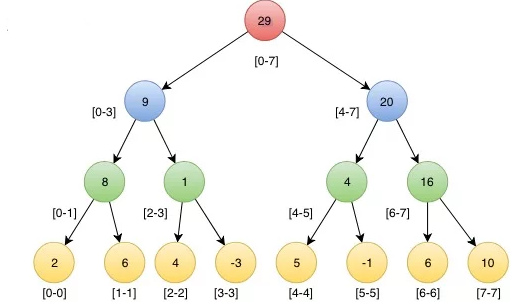
\includegraphics[scale=.50]{./img/segment_tree.png}}
\end{frame}

\begin{frame}{Segment Tree}{caratteristiche}
    Nominiamo i nodi a partire da $1$ per livelli: la radice ha indice $1$, il secondo livello contiene i nodi $2$ e $3$, il terzo livello i nodi $4$, $5$, $6$ e $7$ ...\\
    \pause
    Abbiamo quindi un albero con le seguenti caratteristiche:\pause
    \begin{itemize}
        \item la radice ha indice $1$
        \item il figlio sinistro di un nodo $i$ ha indice $2i$
        \item il figlio destro di un nodo $i$ ha indice $2i + 1$
        \item il padre di un nodo $i$ ha indice $i/2$
        \item i nodi sono numerati da $1$ a $2N - 1$
        \item l'albero ha altezza $O(\log N)$
    \end{itemize}
\end{frame}

\begin{frame}
    \makebox[\textwidth]{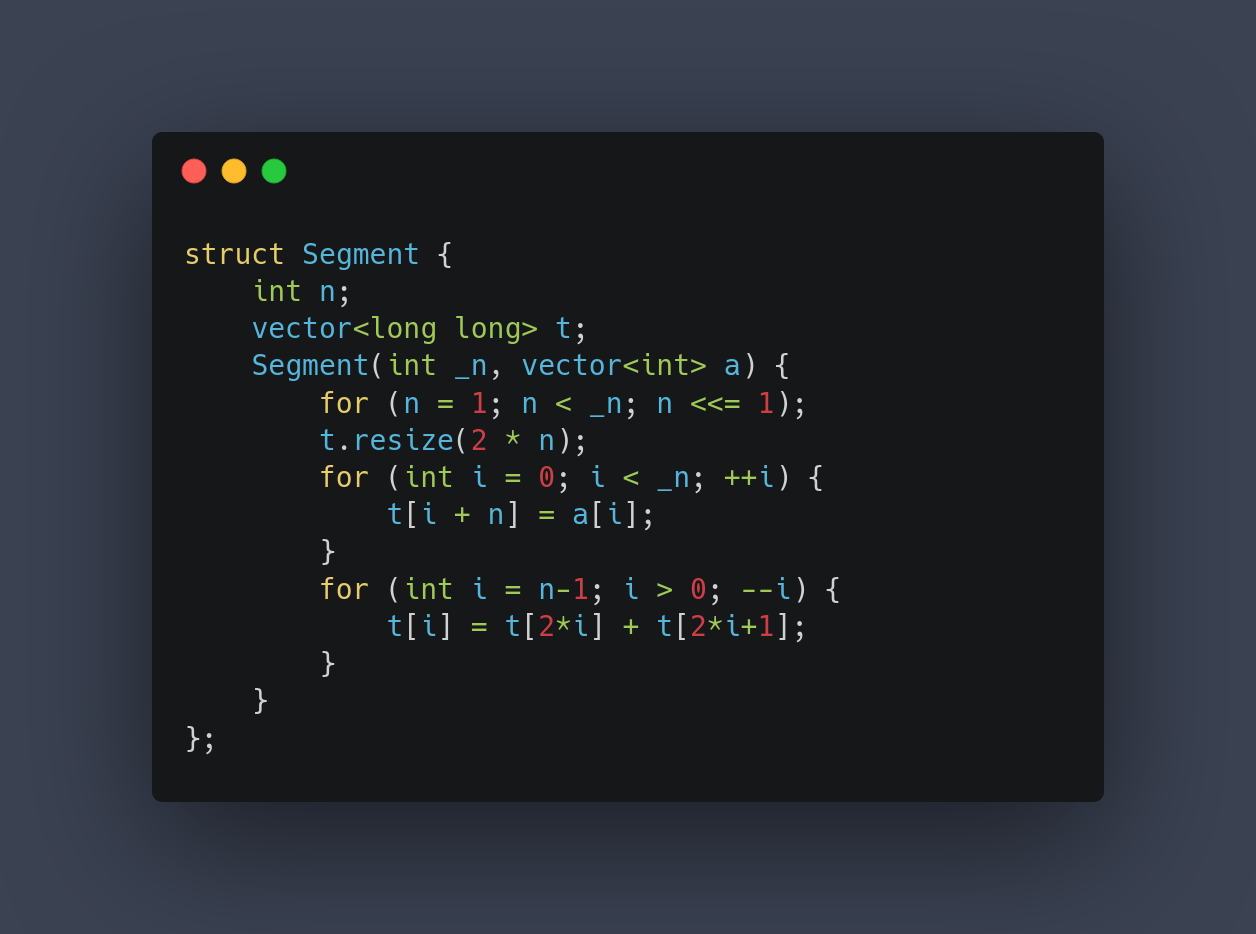
\includegraphics[scale=.3]{./img/st_build.png}}
\end{frame}

\begin{frame}{Segment Tree}{Update}
    Abbiamo definito la struttura del segment tree, ma non sappiamo ancora come utilizzarlo per risolvere il problema.\\
    \pause
    Dobbiamo capire come aggiornare il segment tree e rispondere alle query.\\
    \pause
    Update:\\
    Notiamo che ogni nodo è contenuto in esattamente $\log N $ intervalli, possiamo quindi aggiornarli tutti in $O(\log N)$.
\end{frame}

\begin{frame}
    \makebox[\textwidth]{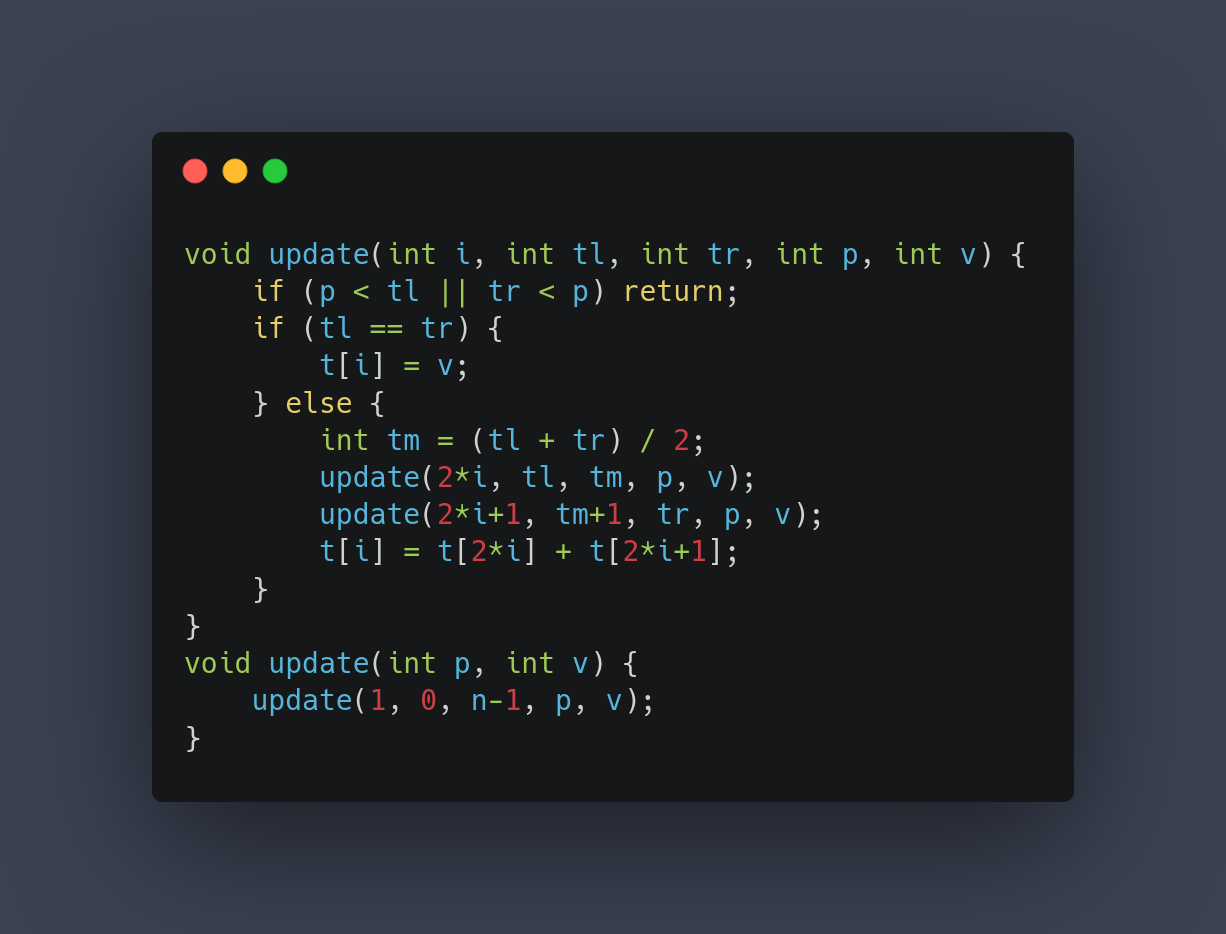
\includegraphics[scale=.3]{./img/st_update_rec.png}}
\end{frame}

\begin{frame}
    \makebox[\textwidth]{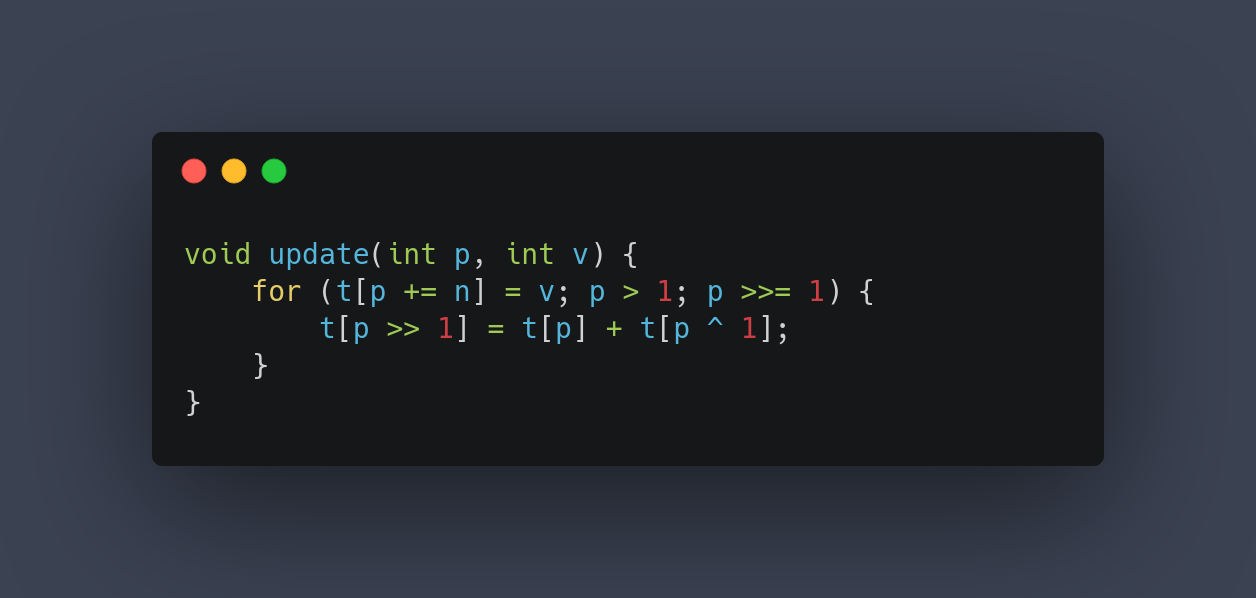
\includegraphics[scale=.3]{./img/st_update.png}}
\end{frame}

\begin{frame}{Segment Tree}{Query}
    La query è un po' più complessa. Dobbiamo trovare un insieme di intervalli da unire per ottenere la risposta desiderata.\\\vfill
    \makebox[\textwidth]{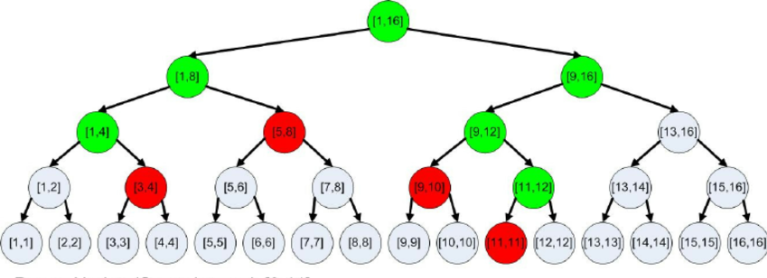
\includegraphics[scale=.40]{./img/query.png}}
\end{frame}

\begin{frame}{Segment Tree}{Query}
    Supponiamo di voler rispondere alla query $[l, r]$.\\
    Possiamo utilizzare una dfs sull'albero. Ogni volta che raggiungiamo un nodo abbiamo $3$ possibilità:\\
    \pause
    \begin{itemize}
        \item l'intervallo è completamente contenuto in $[l, r]$, quindi possiamo aggiungerlo alla risposta e fermarci
        \item l'intervallo è completamente fuori da $[l, r]$, quindi possiamo ignorarlo e fermarci
        \item l'intervallo è parzialmente contenuto in $[l, r]$, quindi ricorriamo nei figli
    \end{itemize}
    \pause
    Quanti nodi visitiamo con questo processo?\\
    \pause
    Si può dimostrare che la complessità è $O(\log N)$.\\
    Abbiamo quindi una soluzione che risolve il problema in $O(\log N)$ per query/update.
\end{frame}

\begin{frame}
    \makebox[\textwidth]{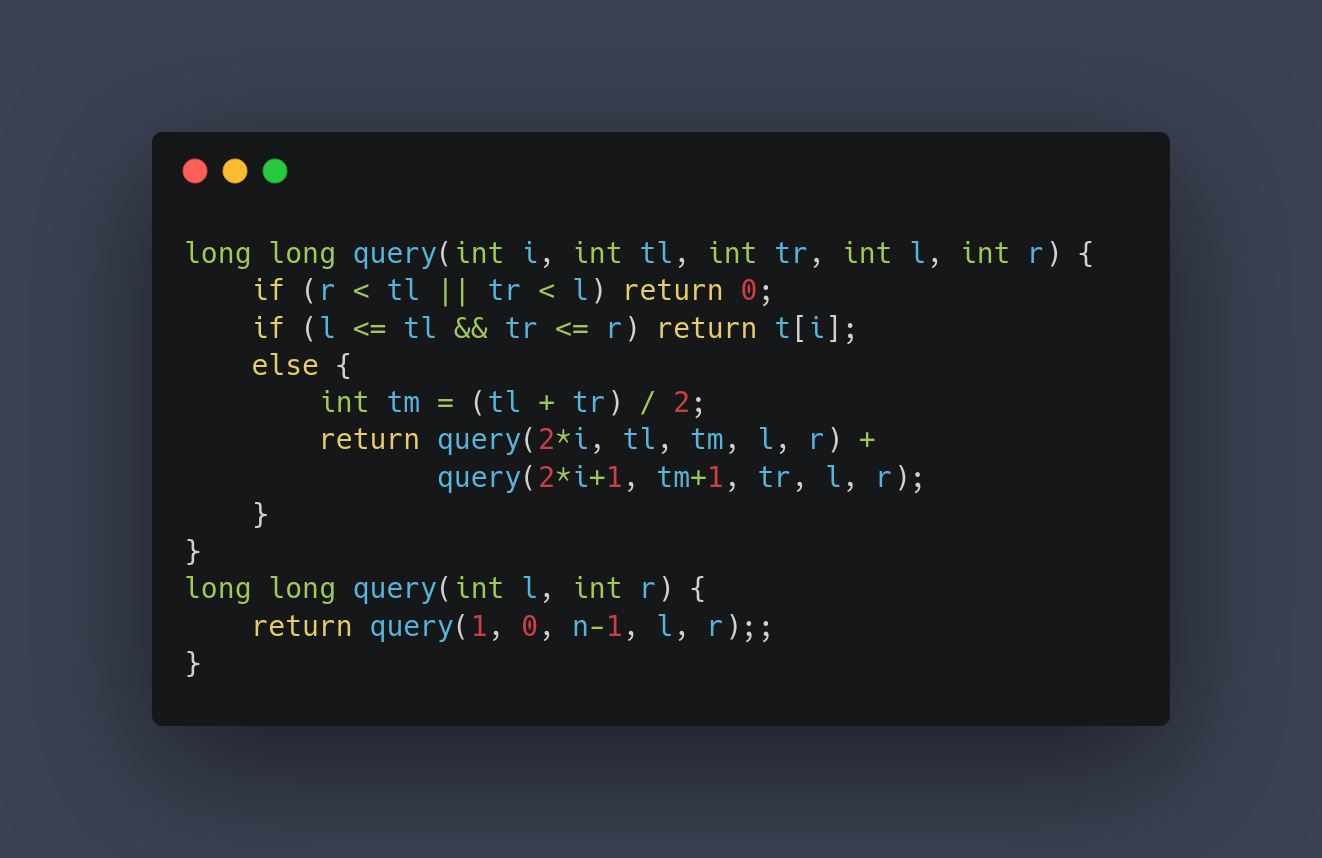
\includegraphics[scale=.3]{./img/st_query.png}}
\end{frame}

\begin{frame}
    Abbiamo visto un segment tree che calcola la somma in un intervallo.\\
    Questa struttura è però molto generica e versatile, possiamo utilizzarla per risolvere molti altri problemi.\\
    \pause
    Un esempio è utilizzarla per rispondere a query di massimo/minimo in un intervallo (come vedremo in un problema).\\
\end{frame}

\section{Problemi}

\subsection{Parkour}
\begin{frame}{Problema}{Parkour}
    \begin{exampleblock}{Pre-Egoi Parkour}
        A Pisa ci sono $N \leq 10^6$ edifici, ognuno dei quali ha altezza $S_i$. Tommaso si trova inizialmente sul tetto dell'edificio $0$ e vuole raggiungere l'edificio $N-1$ \textbf{minimizzando l'altezza massima} dei tetti su cui salta.
        Dalla casa $i$, Tommaso pu\`o raggiungere le case da $i+A_i$ a $i+B_i$ ($1 \leq A_i \leq B_i \forall i$), dove $A,B$ sono array in input.
        Aiuta Tommaso trovando la minima altezza massima per raggiungere $N-1$.
    \end{exampleblock}
    \small{\underline{\url{https://training.olinfo.it/\#/task/pre-egoi-parkour/statement}}}
\end{frame}

\begin{frame}{Problema}{Parkour}
    \begin{itemize}
        \item senza per ora preoccuparci dell'efficienza, cerchiamo una qualunque soluzione (subesponenziale) corretta
        \item idee?
        \pause
        \item immaginiamo di essere sulla casa $i$ e voler raggiungere $N-1$. Sia $dp[i]$ la risposta per questo sottoproblema
        $$dp[i] = \max\left(S_i, \min_{j = i + A_i}^{i + B_i} dp[j]\right)$$
        \item la risposta al problema di partenza \`e $dp[0]$
    \end{itemize}
\end{frame}

\begin{frame}{Problema}{Parkour}
    \vfill
    \begin{itemize}
        \item Ci sono $N$ stati e al momento ogni transizione costa $O(N)$. La complessit\`a attuale \`e $O(N^2)$
        \item abbiamo appena visto una struttura dati in grado di velocizzare significativamente le transizioni!
    \end{itemize}
    \pause
    \makebox[\textwidth]{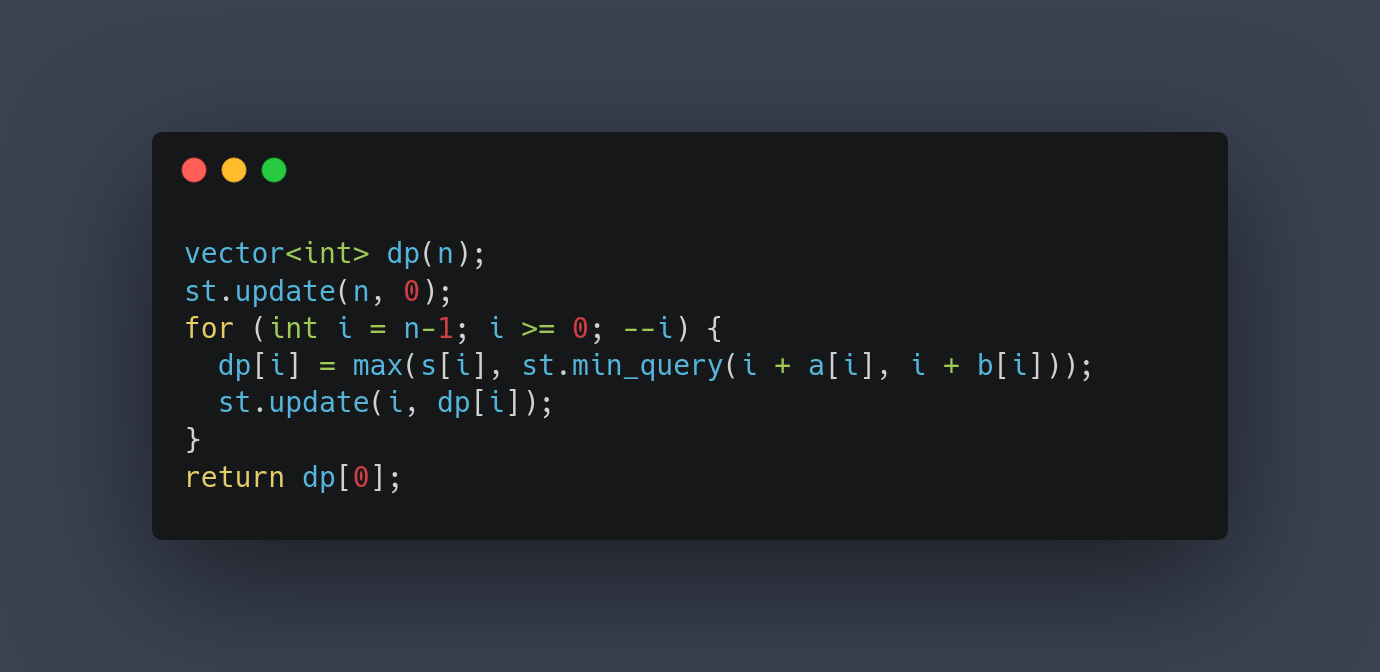
\includegraphics[scale=.3]{./img/parkour.png}}
\end{frame}

\begin{frame}{Problemi}
    \small{\underline{\url{https://cses.fi/problemset/task/1648}}}
    \small{\underline{\url{https://cses.fi/problemset/task/1649}}}
    \small{\underline{\url{https://cses.fi/problemset/task/1650}}}
    \small{\underline{\url{https://cses.fi/problemset/task/2206}}}
    \small{\underline{\url{https://training.olinfo.it/\#/task/pre-egoi-parkour/statement}}}
\end{frame}

\end{document}
